\documentclass[a4paper,10pt,twoside,twocolumn, bg=print]{dndbook} %a4, 10pt, book (idk why i did that...), 2 cols, dnd-themed
\usepackage[english]{babel} %language
\usepackage[utf8]{inputenc} %lovely utf-8
\usepackage{graphicx} %images
\usepackage{wrapfig} %images
\usepackage{tikz} %draw stuff
\usepackage{ifthen} %draw stuff
\usetikzlibrary{shapes,calc,fadings} %draw stuff
\usepackage{xspace} %usefull idk, allways import this stuff
\usepackage{setspace} %don't ask, kind of like it...
\usepackage{pgfplots}

\usepackage[singlelinecheck=false]{caption} %idk dndbook...
\usepackage{listings} %idk dndbook...
\usepackage{shortvrb} %not used yet...
\usepackage{stfloats} %idk dndbook
\usepackage{dirtytalk}

\singlespacing
\makeatletter %because of titlepage and \HUGE

\@openrightfalse %no empty pages

\graphicspath{ {./images/} }

\def \license {GNU Free Documentation License}
\def \licensetext {Please consider and respect the copyleft of this license. The content of this document should be accessible to everyone. Everyone has the right to use the content of this document as he/she wishes, to modify it, to publish it modified (taking into account the copyleft) and to republish it without any changes (taking into account the copyleft).}
\def \author {Sven Hugi}%if you edit this document, add your name... <3
\def \illustrators {Glen Angus and one more} %add name
\def \othercontrib {} %add name


%2 column layout hack...
\newcommand{\nextPage}{
	\newpage
	\hbox{}
	\newpage
}
%make bad things look ok...
\newcommand{\doublelinebreak}{
	\linebreak\linebreak
}
%the old HUGE fontsize
\newcommand\HUGE{\@setfontsize\Huge{60}{80}} 

\renewcommand{\maketitle}{
	\thispagestyle{empty}
	\onecolumn %fuck it
	\vspace*{5cm}
	\begin{center}
		$\vspace*{2cm}$
			{\HUGE\DndFontDropCap{LYTHARI}}\\	
	\end{center}
	\twocolumn %reset shit
}\makeatother

\begin{document}
	\maketitle
	\onecolumn
	\section*{Credits}
	\vspace{.25cm}
	\textbf{Author:} \author\linebreak
	\textbf{Illustrators:} \illustrators\linebreak
	%\textbf{Additional Contributors:} \othercontrib\linebreak
	\textbf{License:} \license\doublelinebreak
	\licensetext\doublelinebreak
	Images (licensed under the Creative Commons license):
	\begin{itemize}
		\item https://static.wikia.nocookie.net/forgottenrealms/images/9/95/Lythari\_mcav4\_54.png/revision/latest (Glen Angus)
		\item https://static.wikia.nocookie.net/eternaldestiny/images/f/f9/Half-elf-girl.jpg/revision/latest (Unknown)
	\end{itemize}
	
	\vfill\hbox{}\vfill\hfill{\tiny This Document was written in \LaTeX.}\twocolumn
	Lythari are good aligned elven lycanthropic wolves often mistaken as werwoves. Lythari differ from werwolves in the fact that they do not have a hybrid form and are friendly when in wolf form. They are born as were-creatures and later bound in a ritual of bounding. This only works if both sides agree to the transformation. This ritual left a scar, which looks like a wolf bite.\linebreak
	They do not like combat and rather use there speed to flee.
	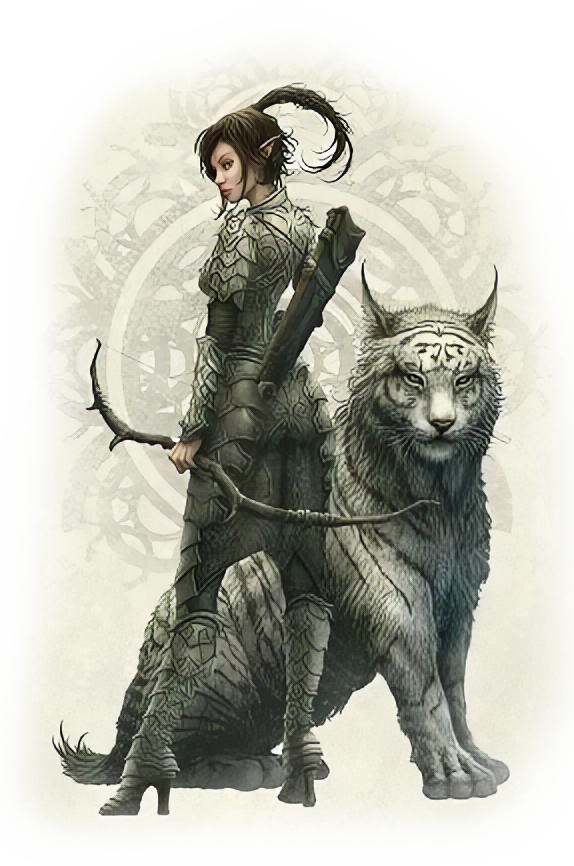
\includegraphics[width=\linewidth]{lythari1.png}
	\section{Lythari Traits}
	\textbf{Ability Score Increase.} Your Dexterity score increases by 2 and your Wisdom score increases by 1.\linebreak
	\textbf{Age.} Although elves reach physical maturity at about the same age as humans, but the elven understanding of adulthood goes beyond physical growth. An elf typically claims adulthood around the age of 100 years and can live to be 750 years old.\linebreak
	\textbf{Alignment.} They are almost always chaotic good and have a high amount of respect for eachother.\linebreak
	\textbf{Size.} Lythari stand around 5 to 6 feet tall and average about 125 pounds. Your size is Medium.\linebreak
	\textbf{Speed.} Your base walking speed is 30ft in your humanoid form and 40ft in wolf form.\linebreak
	\textbf{Language.} You speak Common and Elfen\linebreak
	\textbf{Darkvision.} You can see in dim light within 60 ft of you as if it were bright light, and in darkness as if it were dim light. You can't discern color in darkness, only shades of gray.\linebreak
	\textbf{Wolf Form.} As a Bonus Action you can change between your humanoid form and your wolf form. In your wolf form, you can not use any weapon or shield, only other wolfs and wolf-lycanthropics will understand you and your armor does not count on your ac, you have instead a ac of 12 + your dexterity modifier.\linebreak
	\textbf{Wolf Sense.} In your wolf form, you have an advantage in perception checks that rely on hearing or smelling.\linebreak
	\textbf{Bite.} In your wolf form, your bite acts as a natural weapon, which you can use to make unarmed strikes. If you hit with it, you deal piercing damage equal to 1d6 + your strength modifier instead of the normal damage.\linebreak
	\textbf{Fey Ancestry.} In your humanoid form you have advantage on saving throws against being charmed and magic can't put you to sleep.\linebreak
	\textbf{Trance.} In your humanoid form you do not sleep. Instead you meditate deeply, remaining semi-conscious for 4 hours a day. After resting this way you benefit from the same benefit a human would from 8 hours of sleep.\linebreak
	\textbf{Keen Senses.} You have proficiency in the Perception skill.\linebreak
	
	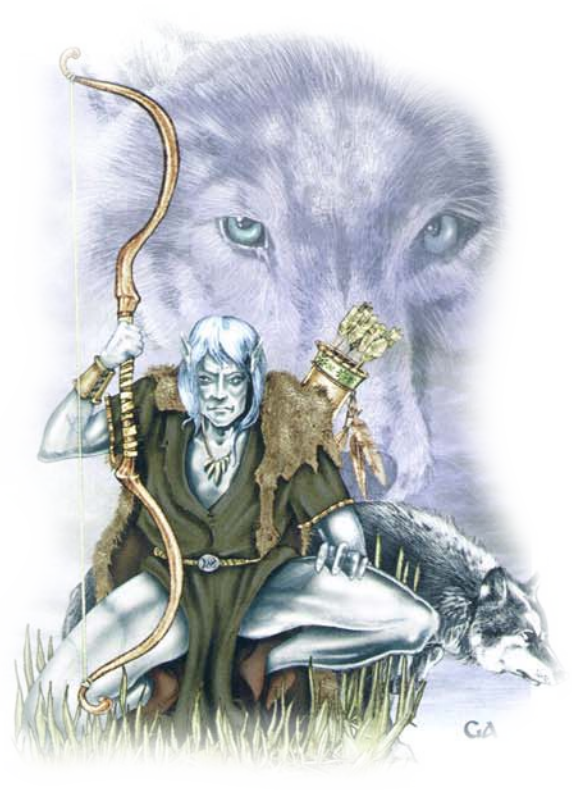
\includegraphics[width=\linewidth]{lythari2.png}
\end{document}